\subsection{Đề xuất bảng khảo sát}
\subsubsection{Đối tượng khảo sát}

Đối tượng được nhắm đến để thực hiện khảo sát bao gồm những người tham gia vào vận hành, thực thi quy trình nghiệp vụ ở những vai trò khác nhau trong quy trình; và những người là khách hàng của quy trình. Như vậy, kết quả chất lượng của quy trình trở nên chính xác và khách quan hơn, vì không chỉ được đánh giá thông qua việc thực thi quy trình trên thực tế, mà còn được đánh giá qua sản phẩm đầu ra của quy trình đó.
\subsubsection{Nội dung khảo sát}

Để đánh giá được toàn diện chất lượng bên ngoài của một quy trình nghiệp vụ, cần phải xem xét đến ba độ đo CES, CSAT, NPS đã được trình bày ở trên. Vì thế, các câu hỏi dùng để thu thập giá trị của những độ đo này là bắt buộc và người thiết kế khảo sát không thể loại trừ chúng ra khỏi bộ câu hỏi. Bài khảo sát tập trung đánh giá trải nghiệm, sự hài lòng của người dùng nên ở đây, nội dung câu hỏi sẽ xoay quanh các yếu tố liên quan đến trải nghiệm của người dùng, đó là thời gian, chi phí, khả năng xử lý ngoại lệ và độ linh hoạt của quy trình.

\par
Tuy nhiên, tuỳ vào loại quy trình mà có sự xuất hiện của đối tượng khách hàng của quy trình hay không. Chẳng hạn như, những quy trình đóng, phục vụ nội bộ thì có thể không xuất hiện đối tượng khách hàng, hay không có một sản phẩm đầu ra cụ thể nào phục vụ cho khách hàng bên ngoài. Vì vậy, người thiết kế bảng khảo sát cần xác định rõ đối tượng khảo sát để tuỳ chỉnh nội dung bảng khảo sát phù hợp, tránh xảy ra tình trạng khảo sát không đúng đối tượng, gây nhầm lẫn và sai lệch kết quả thu được.

\par
Dựa vào những nguyên tắc thiết kế bảng câu hỏi đã được trình bày ở trên, chúng tôi quyết định chọn trình tự các câu hỏi như sau:
\begin{itemize}
    \item Mở đầu bằng những câu hỏi rẽ nhánh, lấy thông tin cơ bản của người dùng, với mục đích lấy kết quả trả lời của người dùng ở những câu hỏi này để điều hướng tới các câu hỏi phù hợp. Thông tin cơ bản của người dùng chỉ bao gồm vai trò cụ thể của người dùng trong quy trình nghiệp vụ đó là gì, là một dạng thông tin công khai.
    \item Nhóm các câu hỏi chung chủ đề lại với nhau, bao gồm các nhóm câu hỏi về CES, CSAT, NPS tương ứng với ba độ đo đã đề cập, với thứ tự như trên, với mục đích sau khi đã tìm hiểu những nỗ lực của người dùng khi thực thi quy trình, sẽ đánh giá sự hài lòng tổng quan đối với quy trình, và cuối cùng là liệu người dùng có muốn đề xuất quy trình cho người khác hay không. Ở trong mỗi nhóm câu hỏi, sẽ đi từ những câu hỏi đánh giá tổng quan trước (được dùng để tính điểm độ đo), sau đó là những câu hỏi để lấy thêm thông tin xoay quanh lựa chọn của người dùng ở những câu hỏi đánh giá tổng quan đó.
\end{itemize}
% \par
% Trong trường hợp phạm vi nghiệp vụ của người dùng không có ngoại lệ nào cần xử lý, hoặc không có ngữ cảnh nào được xem xét, trước khi đi vào khảo sát chi tiết, ta có thể có câu hỏi để kiểm tra xem trong phạm vi lane của họ có ngoại lệ hay ngữ cảnh nào đã được mô tả hay chưa. Tuỳ thuộc vào câu trả lời, ta sẽ dẫn người dùng đến với những câu hỏi phù hợp.
\subsubsection{Hình thức câu hỏi}

Chúng tôi sẽ sử dụng một số hình thức câu hỏi khác nhau. Điều này cho phép chúng tôi có thể thu thập nhiều hơn thông tin từ người dùng. Dưới đây là bảng các hình thức và tên câu hỏi được sử dụng trong bài khảo sát:
\begin{table}[H]
    \def\arraystretch{2}%
    \centering
    \resizebox{\textwidth}{!}{
        \begin{tabular}{|p{4cm} |p{8cm} |p{2cm}|}
            \hline
                Hình thức  & Mô tả & Ký hiệu \\ [0.5ex]
            \hline
                Multiple choice (single select) question & 
                Nhiều lựa chọn, nhưng một lúc chỉ chọn nhiều nhất một đáp án &
                MC - SS \\
            \hline
                Open question & 
                Cho phép nhập câu trả lời tuỳ ý, dưới dạng một đoạn văn ngắn hoặc câu trả lời ngắn & 
                OP \\
            \hline
                Likert Scale question & 
                Dùng để đánh giá CES, NPS, CSAT với các mức độ khác nhau & 
                LS \\
            \hline
                Dichotomous & 
                Hai lựa chọn, cùng lúc chỉ chọn một đáp án & 
                DM \\ [1ex] 
            \hline
        \end{tabular}
    }
    \caption{Các hình thức câu hỏi được sử dụng trong bảng khảo sát}
\end{table}

\par
Chúng tôi cũng đặt tên các câu hỏi theo mục đích của chúng.
\begin{table}[H]
    \def\arraystretch{2}%
    \centering
    \resizebox{\textwidth}{!}{
        \begin{tabular}{|p{4cm} |p{8cm} |p{2cm}|}
            \hline
                Tên  & Mô tả & Ký hiệu \\ [0.5ex] 
            \hline
                CES question & 
                Câu hỏi đánh giá điểm CES & 
                CES \\
            \hline
                CSAT question & 
                Câu hỏi đánh giá điểm CSAT & 
                CSAT \\
            \hline
                CES insight question & 
                Câu hỏi thu thập thêm thông tin từ việc đánh giá CES của người dùng & 
                CES - IN \\
            \hline
                CSAT insight question & 
                Câu hỏi thu thập thêm thông tin từ việc đánh giá CSAT của người dùng & 
                CSAT - IN \\
            \hline
                NPS question & 
                Câu hỏi đánh giá điểm NPS & 
                NPS \\ 
            \hline
                User-information-collecting question & 
                Câu hỏi thu thập thông tin cơ bản của người dùng & 
                UIC \\
            \hline
                Branching question & 
                Câu hỏi điều kiện, mục đích điều hướng người dùng tới những câu hỏi khác phù hợp với câu trả lời của họ ở câu hỏi này & 
                BR \\ [1ex]
            \hline 
        \end{tabular}
    }
    \caption{Tên các câu hỏi được sử dụng trong bảng khảo sát}
\end{table}

\subsubsection{Nội dung câu hỏi}

\textbf{Câu hỏi điều kiện:}
\begin{itemize}
    \item Do you use any products or services provided by this process?
    \item Are there any handled exceptions in your process?
    \item Variations refer to process’ workflows in different conditions. Are there any variations in your process?
\end{itemize}
\par
Các câu hỏi điều kiện được sử dụng để xác định chi tiết đối tượng của bài khảo sát, liệu trong phần quy trình của họ có xảy ra những ngoại lệ nào đã được xử lý hay không, hay có bất kỳ những biến thể của quy trình hay không. Với những thông tin cung cấp từ người dùng sẽ điều hướng họ tới những câu hỏi sau đó phù hợp với câu trả lời ở những câu hỏi này.

\textbf{Câu hỏi lấy thông tin cơ bản của người dùng:}
\begin{itemize}
    \item What is your role in this process?
\end{itemize}
\par
Câu hỏi này dùng để xác định xem vai trò cụ thể của người dùng (lane) trong quy trình nghiệp vụ là gì, sau khi người dùng được phân loại thuộc nhóm những người tham gia vận hành, thực thi quy trình.

\textbf{Câu hỏi CES}
\begin{itemize}
    \item To what extent do you agree with this statement: “It is easy to handle exceptions in your process”.
    \item To what extent do you agree with this statement: “It is easy to execute your process”.
\end{itemize}
\par
Hai câu hỏi CES tập trung đánh giá nỗ lực của người dùng trong việc thực thi quy trình nói chung, và xử lý những ngoại lệ xảy ra trong quá trình thực thi đó. Người dùng đồng ý với mệnh đề ở mức độ nào sẽ chọn giá trị tương ứng trong những lựa chọn được cung cấp sẵn.
Ngoài ra, để thu thập thêm thông tin xoay quanh những ngoại lệ xảy ra trong quy trình, chúng tôi cung cấp thêm một số câu hỏi theo sau (follow-up question), nhưng những câu hỏi này không được sử dụng để tính điểm khảo sát:
\begin{itemize}
    \item How frequently do exceptions happen in practice?
    \item Which handled exceptions do you think the way to handle them needs optimizing? Can you suggest some solutions to those?
    \item Can you suggest any exceptions that need handling and the way to handle them?
\end{itemize}
\par
Các câu hỏi trên tìm hiểu nhiều hơn về việc người dùng nhận thấy những ngoại lệ trên thực tế xảy ra với tần suất như thế nào. Trong số những ngoại lệ đã được xử lý bởi người thiết kế quy trình, người dùng có cảm thấy cách xử lý nào chưa được tối ưu hay vẫn còn một số vấn đề như quá phức tạp, tốn nhiều thời gian không, và họ có thể đề xuất những giải pháp khác. Bên cạnh đó, người dùng có gặp phải những ngoại lệ mà chưa được xử lý không, và trong những trường hợp đó, người dùng đã làm gì để giải quyết tạm thời. Sau khi thu thập được những thông tin này, người thiết kế quy trình nghiệp vụ có thể đưa ra được các phương án để tối ưu quy trình và xử lý các ngoại lệ có thể có.

\textbf{Câu hỏi CSAT}
\begin{itemize}
    \item How satisfied are you with the way exceptions are handled in your process?
    \item A flexible process means it has suitable variations for different conditions. How satisfied are you with those variations of the process?
    \item How satisfied are you with the amount of time you have to spend on this process?
    \item How satisfied are you with the cost of products or services of this process?
    \item How satisfied are you with the products or services provided by this process?
    \item How satisfied are you with the total time you have to spend on waiting for the output of this process?
\end{itemize}
\par
Các câu hỏi CSAT tập trung đo lường mức độ hài lòng của người dùng ở cách các ngoại lệ đã được xử lý trong quy trình, việc quy trình có những biến thể để linh hoạt đáp ứng các điều kiện khác nhau xảy ra trong quá trình thực thi, thời gian, chi phí mà người dùng phải bỏ ra để thực thi quy trình, cũng như kết quả đầu ra của quy trình. Người dùng cảm thấy hài lòng tới mức độ nào thì có thể chọn giá trị tương ứng trong những lựa chọn được cung cấp sẵn. Ngoài ra, chúng tôi đề xuất thêm câu hỏi theo sau để tìm hiểu xem liệu người dùng có gặp vấn đề khi sử dụng sản phẩm hoặc dịch vụ mà quy trình nghiệp cung cấp hay không. Từ đó, người thiết kế quy trình nghiệp vụ có thể đưa ra những giải pháp để nâng cao chất lượng sản phẩm, dịch vụ của quy trình.Và câu hỏi này không được dùng để tính điểm CSAT:
\begin{itemize}
    \item Do you encounter any problems while using products or services provided by this process?
\end{itemize}
\par
\textbf{Câu hỏi NPS}
\begin{itemize}
    \item How likely is it that you would recommend this process to others?
\end{itemize}
\par
Để chốt lại bảng khảo sát, câu hỏi NPS sẽ được sử dụng để đánh giá liệu người dùng có cảm thấy quy trình nghiệp vụ xứng đáng để được giới thiệu cho những người khác hay không. Người dùng có thể chọn câu trả lời phù hợp với đánh giá và thái độ của họ.
\par
Để có cái nhìn tổng quan nhất về những câu hỏi trong bảng khảo sát, chúng tôi xin cung cấp bảng tổng hợp các câu hỏi cũng như trình tự các câu hỏi được thể hiện dưới dạng biểu đồ như sau:

\begin{table}[H]
    \def\arraystretch{2}%
    \centering
    \resizebox{\textwidth}{!}{
        \begin{tabular}{|p{0.8cm} |p{1.5cm} |p{1cm}| p{0.8cm} | p{5cm} | p{5cm} |}
            \hline
                Câu hỏi  & Hình thức & Thang điểm & Tên & Nội dung & Bản dịch (tiếng Việt)\\ [0.5ex] 
            \hline
                Q1 & DM &  & BR & Do you use any products or services provided by this process? & Bạn có sử dụng sản phẩm hay dịch vụ nào được cung cấp bởi quy trình này không? \\
            \hline
                Q2 & MC - SS &  & UIC & What is your role in this process? & Vai trò của bạn trong quy trình này là gì? \\ 
            \hline
                Q3 & DM &  & BR & Are there any handled exceptions in your process? & Trong quy trình của bạn có xảy ra ngoại lệ nào đã được xử lý không? \\
            \hline
                Q4 & DM & & BR & Variations refer to process’ workflows in different conditions. Are there any variations in your process? & Các biến thể là các luồng thực thi ở những điều kiện khác nhau của quy trình. Trong quy trình của bạn, có xảy ra biến thể nào của quy trình hay không? \\
            \hline
                Q5 & LS & 1 - 7 & CES & To what extent do you agree with this statement: “It is easy to handle exceptions in your process”. & Bạn đồng ý với mệnh đề này tới mức độ nào: “Bạn cảm thấy dễ dàng để xử lý các ngoại lệ trong quy trình nghiệp vụ”. \\
            \hline
                Q6 & LS & 1 - 7 & CES & To what extent do you agree with this statement: “It is easy to execute your process.” & Bạn đồng ý với mệnh đề này tới mức độ nào: “Bạn cảm thấy dễ dàng thực thi quy trình nghiệp vụ”. \\
            \hline
                Q7 & MC - SS &  & CES - IN & How frequently do exceptions happen in practice? & Hãy chọn mức độ thường xuyên xảy ra ngoại lệ trên thực tế theo đánh giá của bạn. \\
            \hline
                Q8 & OP & & CES - IN & Which handled exceptions do you think the way to handle them needs optimizing? Can you suggest some solutions to those? & Trong số những ngoại lệ đã được xử lý, bạn nghĩ cái nào cách xử lý của nó vẫn chưa được tối ưu? Bạn có thể đề xuất một số cách tối ưu của bạn cho ngoại lệ đó được không? \\
            \hline
                Q9 & OP & & CES - IN & Can you suggest any exceptions that need handling and the way to handle them? & Bạn có thể đề xuất một số những ngoại lệ cần phải được xử lý và cách xử lý chúng không? \\ [1ex]
            \hline
        \end{tabular}
    }
\end{table}

\begin{table}[H]
    \def\arraystretch{2}%
    \centering
    \resizebox{\textwidth}{!}{
        \begin{tabular}{|p{0.8cm} |p{1.5cm} |p{1cm}| p{0.8cm} | p{5cm} | p{5cm} |}
            \hline
                Q10 & LS & 1 - 7 & CSAT & A flexible process means it has variations for different conditions. How satisfied are you with those variations of the process? & Một quy trình được xem là linh hoạt khi nó có nhiều biến thể cho nhiều điều kiện khác nhau. Bạn hài lòng như thế nào với những biến thể này của quy trình? \\
            \hline
                Q11 & LS & 1 - 7 & CSAT & How satisfied are you with the way exceptions are handled in your process? & Bạn hài lòng như thế nào với cách mà quy trình nghiệp vụ xử lý các ngoại lệ? \\
            \hline
                Q12 & LS & 1 - 7 & CSAT & How satisfied are you with the amount of time you have to spend on this process? & Bạn hài lòng như thế nào với tổng thời gian bạn dành cho quy trình? \\
            \hline
                Q13 & LS & 1 - 7 & CSAT & How satisfied are you with the cost of products or services of this process? & Bạn hài lòng như thế nào với chi phí của sản phẩm, dịch vụ của quy trình? \\
            \hline
                Q14 & LS & 1 - 7 & CSAT & How satisfied are you with the products or services provided by this process? & Bạn hài lòng như thế nào với sản phẩm, dịch vụ quy trình cung cấp? \\
            \hline
                Q15 & LS & 1 - 7 & CSAT & How satisfied are you with the total time you have to spend on waiting for the output of this process? & Bạn hài lòng như thế nào với thời gian chờ sản phẩm hay dịch vụ của quy trình? \\
            \hline
                Q16 & OP &  & CSAT - IN & Do you encounter any problems while using products or services provided by this process? & Bạn có gặp vấn đề gì trong quá trình sử dụng sản phẩm, dịch vụ của quy trình không? \\
            \hline
                Q17 & LS & 0 - 10 & NPS & How likely is it that you would recommend this process to others? & Bạn có muốn đề xuất quy trình nghiệp vụ này cho người khác không? \\ [1ex]
            \hline
        \end{tabular}
    }
    \caption{Tổng hợp các câu hỏi trong bảng khảo sát}
\end{table}

\begin{figure}[H]
    \centering
    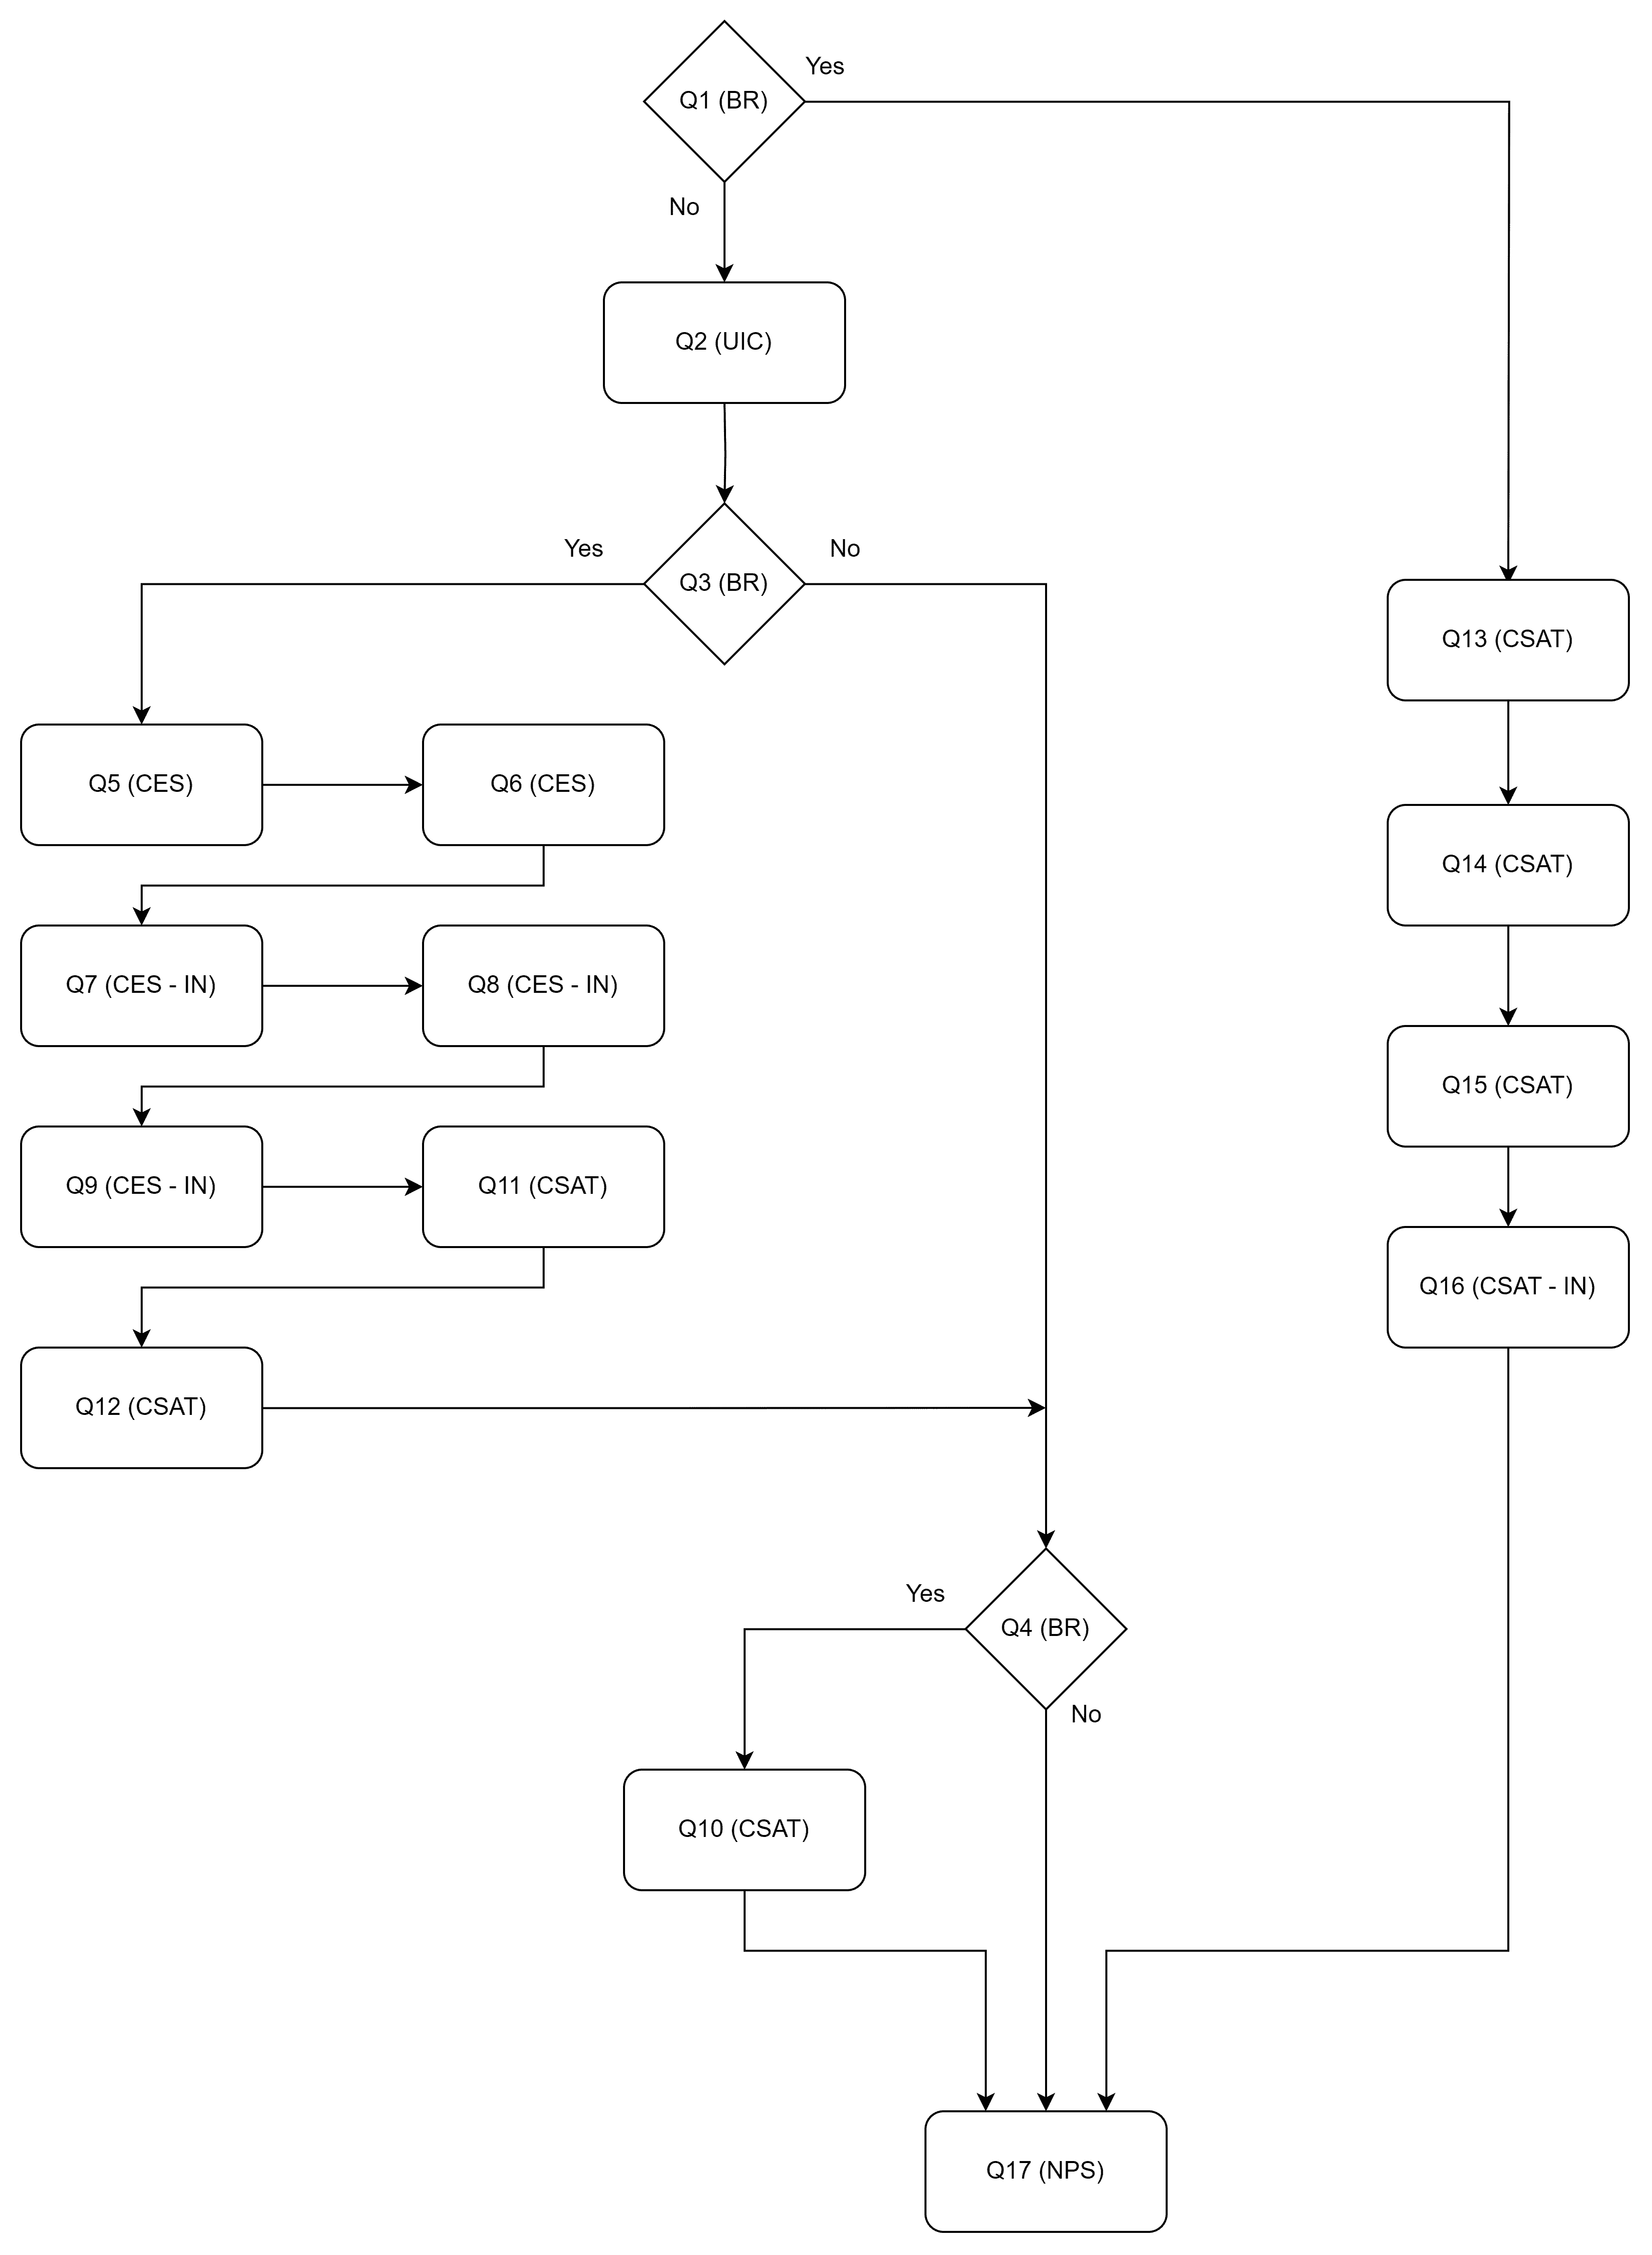
\includegraphics[width = \linewidth]{Content/Cơ sở lý thuyết/documents/Survey/images/surveyflow.png}
    \vspace{0.5cm}
    \caption{Lược đồ trình tự câu hỏi trong bảng khảo sát}
    \label{fig:Lược đồ trình tự câu hỏi trong bảng khảo sát}
\end{figure}